\chapter{Desenvolvimento do concreto}

A história do desenvolvimento do concreto tem pelo menos 20 séculos, até chegar a ser o produto industrializado mais consumido no mundo atual. Tamanha popularidade deve-se, principalmente, à disponibilidade de matéria-prima em praticamente todos os continentes, além de sua versatilidade, durabilidade e bom desempenho como material construtivo e competitividade econômica, frente à outros materiais de construção.

Este capítulo é dedicado a apresentar um breve histórico do desenvolvimento do concreto, desde seus primórdios aos dias atuais.

\section{Início do desenvolvimento do concreto}

O Homem sempre fez uso dos materiais disponíveis na natureza para satisfazer suas necessidades de sobrevivência e abrigo. \apudonline{Cohen}{Isaia} aponta que um desses primeiros materiais foi a argila, utilizada  para construir utensílios domésticos e abrigos mais resistentes. Segundo \apudonline{Mali}{Isaia}, em seguida passou-se a utilizar cal e gesso para revestimento de pisos e paredes, como pôde ser verificado em antigas cidades do Oriente Médio \cite{Isaia}.

Os gregos já dominavam o processo empírico de produção de cal hidráulica e de concreto já no século V a.C. \apudonline{Koui}{Isaia} analisaram uma cisterna de concreto construída em Kamiros, ilha de Rodes, Grécia, construída por volta dessa época, e descobriram que o traço granulométrico utilizado se aproxima muito da curva granulométrica ideal de Füller. Este concreto é constituído de seixo rolado, calcário médio e fino, terra vulcânica e cal e possui uma resistência característica de 13,5 MPa, um resultado notável para um material feito há mais de 2500 anos. Ainda assim, as grandes construções gregas eram, predominantemente, feitas com pedras. Foram os romanos que aperfeiçoaram o uso do concreto e passaram a aplicá-lo em pilares, vigas, abóbodas e cúpulas de grandes dimensões. Vitrúvio (1 a.C.), em seu livro De Archtectura, mostra que a composição do concreto romano consistia de argila caulinítica calcinada ou pedras vulcânicas calcinadas e areia vulcânica reativa, de origem natural \cite{Isaia}.

O desenvolvimento da tecnologia do concreto passou por um grande hiato durante a Idade Média, o qual só retorna na época do Renascimento (século XIV), marcando o início da Idade Moderna. É importante notar que foi nesse período que Galileo Galilei começou a dar as bases para o que viria a se tornar a engenharia de vigas, além de outras figuras importantíssimas para a ciência dos materiais, como Robert Hooke e sua teoria da elasticidade dos corpos, Isaac Newton e a inauguração da física clássica e, assim como Leibni, contribuíram para o desenvolvimento cálculo integral e diferencial, formando a base teórica para o entendimento das leis fundamentais que regem as estruturas \cite{Isaia}.

Logo após a Revolução Industrial, diversos tipos de cimento foram patenteados, porém o que obteve mais sucesso foi o cimento Portland, patenteado em 1824 pelo inglês Joseph Aspdin. Este material só foi chegar ao Brasil em 1855, trazido pelo comendador Antônio Proost Rodovalho \cite{Isaia}.

O cimento Portland consiste basicamente da mistura de clínquer moído e gesso. Clínquer é um material obtido a partir da mistura e moagem de pedras calcárias, margas e britas de rochas, as quais são colocadas em fornos rotativos e submetidas a temperaturas superiores a 1400\textsuperscript{\degree} C. O cimento ainda pode receber alguns aditivos, que podem agregar algumas características como resistência a sulfatos, baixo calor de hidratação, entre outras.

No século XIX houve um grande salto no desenvolvimento da tecnologia do concreto, resultando no tão popular concreto armado. Lambot, um agricultor francês, começou a utilizar cimento com telas de ferro para fazer tanques e em 1855, apresentou um barco construído com essa técnica em Paris, patenteando o método. Monier, um jardineiro francês, observou o barco e passou a construir vasos com a mesma técnica, a qual evoluiu e começou a produzir painéis de fachada, o que patenteou em 1867. Em 1875, Monier construiu a primeira ponte de concreto armado do mundo, no castelo de Chazelet, França \autoref{chazelet}. Com 18,80 m de comprimento e 4,25 m de largura, a ponte é a realização do conhecimento empírico e intuitivo de Monier ao empregar aço e concreto para sua construção.

\begin{figure}[htb]
	\caption{\label{chazelet}Ponte de concreto armado sobre o fosso do castelo de Chazelet, França. Construída por Joseph Monier em 1875.}
	\begin{center}
		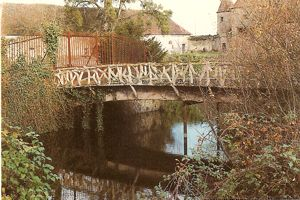
\includegraphics[max width=\textwidth]{Monier_bridge_Chazelet.jpg}
	\end{center}
	\fonte{\citeonline{chazelet}.}
\end{figure}

Monier vendeu suas patentes de concreto armado em 1884 para duas empresas alemãs, que posteriormente foram vendidas para o engenheiro alemão Gustav Wayss em 1886, da empresa Wayss \& Freytag. Wayss passou a investir em pesquisa e um de seus funcionários, Mörsch, foi quem aprimorou e estabeleceu bases científicas para o concreto armado, escrevendo o livro intitulado ``Der Betoneisenbau: Seine theorie und Anwendung'' (Construções de Concreto e Aço: Sua teoria e aplicação).

O primeiro edifício em concreto armado feito no Brasil foi construída pela Wayss \& Freytag em 1907, na rua São Bento, em São Paulo - SP. Possuía apenas três pavimentos, mas já era um marco para a época.

Os primeiros estudos acerca de concreto protendido começaram na década de 20, possibilitando a construção de estruturas mais esbeltas, leves e capazes de vencer vãos maiores do que o concreto armado é capaz de suportar.

A popularidade do concreto deve-se, principalmente, às seguintes características:

\begin{alineas}[label=\textbullet]
  \item Disponibilidade de matéria prima: 89\% da crosta terrestre é formada por 90\% dos materiais que compõem o concreto;
  \item Versatilidade na modelagem: em seu estado fresco é um material plástico, se adequando a qualquer forma desejada;
  \item Sólido: depois da cura, se torna um material, praticamente homogêneo, solidarizado entre si;
  \item Durável: tomadas as devidas precauções, o concreto é capaz de resistir aos efeitos do tempo e do ambiente;
  \item Custo: por conta da disponibilidade de matéria prima e bom desempenho, é um material extremamente competitivo na cadeia de materiais de construção civil;
  \item Sustentabilidade: quando bem executadas, as estruturas de concreto são muito duráveis, é um material facilmente encontrado e de produção regional, utiliza rejeitos industriais como adição e seu entulho é totalmente reciclável.
\end{alineas}

Apesar disso, o concreto ainda possui algumas desvantagens, como baixa resistência à tração, elevado peso próprio, acentuada variação volumétrica e dificuldade na moldagem de peças de grande volume, devido ao calor gerado na hidratação. Cada um destes problemas tem uma solução específica, a ser determinada pelo projetista.

\section{Tecnologias de construções de concreto}

O concreto, quando não associado a nenhum outro material, é denominado concreto simples. O concreto simples é incapaz de suportar seu próprio peso, já que o material possui uma capacidade de resistência à tração muita baixa (cerca de 10\% de sua resistência a compressão), de modo que, para se construir edificações, é necessário associá-lo a outras materiais, sendo o método mais comum e difundido, a associações do concreto com o aço. As seguintes seções apresentam mais detalhes desta associação e da industrialização do método.

\subsection{Concreto armado}

Concreto armado é um material de construção civil que consiste na combinação do concreto simples com uma armadura de aço. O concreto resiste aos esforços de compressão aos quais a estrutura será solicitada e fornece ao aço um ambiente alcalino que o protege dos efeitos corrosivos do ambiente, dado uma espessura mínima de cobrimento de concreto sobre a armadura. Por sua vez, o aço (após a fissuração inicial do concreto) resiste aos esforços de tração aos quais a estrutura é solicitada, o que ocorre devido à aderência de uma material ao outro. Outro fator determinante para a escolha destes dois materiais são os seus respectivos valores do coeficiente de dilatação térmica, próximos entre si, o que garante que as deformações térmicas sofridas pelo aço são praticamente iguais à do concreto.

A armadura de aço contida nos elementos estruturais de concreto armado é chamada de armadura passiva, pois ele só começa a ser solicitada quando algum carregamento é adicionado à estrutura. O concreto, por sua vez, incapaz de suportar os esforços de tração, fissura e, por conta da aderência da interface concreto-aço, os esforços são transmitidos à armadura, a qual passa a resistir aos esforços de tração.

\subsection{Concreto protendido}

Concreto protendido é um material de construção civil que consiste na combinação de concreto simples com cabos de aço protendido, isto é, pré ou pós tensionado. Estes cabos comprimem o concreto, o qual não fissura na iminência de um carregamento que gere esforços de tração, já que os cabos protendidos recebem estes carregamentos de maneira ativa, diferentemente do concreto armado, onde a armadura age de maneira passiva. Desse modo, a protensão diminui ou anula as solicitações de tração no concreto e ainda melhora a resistência ao cisalhamento e à torção da peça estrutural.


\subsection{Concreto pré-moldado}

O concreto pré-moldado é uma peça estrutural ou decorativo produzida de maneira industrializada, os quais, posteriormente, são transportados para montagem final. O seu processo de produção visa diminuir o tempo de construção e mobilização de trabalhadores no canteiro de obras.
 
\section{Concretos especiais}

O século XX foi marcado pela busca da otimização dos processos de produção e de projeto de estrutura de concreto, mas ao que tudo indica, o século XXI será marcado pela busca otimização do concreto em si, afim de torná-lo um material ainda mais barato, versátil e capaz de competir ainda mais com o aço na construção civil. Nesta seção, apresenta-se as últimas tecnologias disponíveis para o uso de concreto na construção civil:

\begin{alineas} %[label=\textbullet]
  \item \textbf{Concreto de alto desempenho (CAD):} trata-se de uma classe de concreto com resistências superiores ao concreto convencional, de 40 MPa a 100 MPa;
  
  \item \textbf{Concreto de ultra alto desempenho (CUAD):} trata-se de uma nova classe de concretos especiais. Este trabalho expõe este material em detalhes no \autoref{chap:CUAD};
  
  \item \textbf{Concreto com aditivos especiais:} aditivos são materiais que, adicionados ao concreto, são capazes de mudar seu comportamento fisíco e/ou químico, de acordo com a necessidade da construção. Abaixo, lista-se alguns exemplos de aditivos disponíveis no mercado e suas características:
    \begin{incisos}
      \item \textbf{Acelerador de pega:} para uma moldagem rápida e consequente breve desforma;
      
      \item \textbf{Adição de minerais pozolânicos:} este aditivo é obtido em regiões de atividade vulcânica ou feito artificialmente em fornos industriais. Dos aditivos desta categoria, o principal é a cinza volante, utilizada para retardar a hidratação do concreto e diminuir sua reação álcali-agregado, retartando o ganho inicial de resistência mecânica e diminuindo a quantidade de calor liberado durante a hidratação. Com isso, a incidência de fissuras em peças volumosas de concreto é inibida;
      
      \item \textbf{Aditivos diminuidores ou compensadores de retração:} esses aditivos visam resolver o mesmo problema: retração do concreto e empenamento das placas de piso;
      
      \item \textbf{Aditivos tensoativos:} ajuda a incorporar ar no concreto, diminuindo a tensão superficial que a água causa. Assim reduz a segregação e exsudação, mas diminuindo a resistência mecânica;
      
      \item \textbf{Plastificantes/redutores de água:} aumenta a trabalhabilidade do concreto sem a necessidade de se adicionar mais água. A adição desse material é de 0,2 a 0,7\% da massa de cimento, e pode representar cerca de 20\% na redução de água na pasta;
      
      \item \textbf{Rebarbas metálicas e carbono:} visa transformar o concreto em um material condutor de eletricidade, utilizando a própria peça estrutural para aquecer o ambiente ou derreter gelo e neve em áreas externas;
      
	  \item \textbf{Retardador de pega:} assim como o nome já diz, aumenta o tempo disponível para se trabalhar com o concreto. Muito utilizado durante concretagens demoradas e locais de clima quente. Pode retardar o início da pega em até 8 horas;
    \end{incisos}
    
    \item \textbf{Concreto com fibras:} a adicão de fibras ao concreto tem como finalidade redistribuir de maneira mais uniforme os esforços a qual a peça estrutural é solicitada, predominantemente na seção de tração, pois aumenta seu módulo de elasticidade sem diminuir sua resistência mecânica. Sua aplicação é mais comum em rodovias, pisos industriais e pistas de aeroportos. As fibras podem ser de aço, polipropileno, vidro, carbono, poliéster e nylon, entre outras;
    
    \item \textbf{Concreto leve estutural:} o concreto leve estrutural substitui o agregado comum por agregados leves (pedra pomes, escória vulcânica, argila expandida e escória expandida), fazendo com que sua massa específica seja 20\% menor que a do concreto convencional. Por conta de empregar o uso de agregados porosos, estruturas feitas com concreto leve estrutural sofrem de deformações mais acentuadas, já que seu módulo de elasticidade varia de 50\% a 80\% do concreto convencional. O agregado leve também tende a se acumular na superfície durante a concretagem, além de absorver água, fator que deve ser levado em consideração na hora de se determinar o traço do concreto. O acúmulo do agregado na superfície pode ser controlado com os agregados miúdos;
    
    \item \textbf{Concreto arquitetônico e decorativo:} 
    o concreto sem fim estrutural ou também conhecido como arquitetônico, tem mesmo desempenho de um concreto convencional. Pigmentos inertes podem ser adicionados para dar coloração ao concreto;
    
   
    \item \textbf{Concreto para blindagem de radiação:} utiliza-se agregados pesados, como hematita, de acordo com a intensidade da radiação a qual estará exposto;
    
    \item \textbf{Concreto fotocalítico:} com a incorporação de dióxidos de titânio ou silício em sua composição ou em sua superfície, é possível transformar gases nocivos, como óxido de nitrogênio em nitratos essenciais para o desenvolvimento das plantas, através da fotocálise;
    
    \item \textbf{Concreto autocicatrizante:} incorpora-se bactérias capazes metabolizar os componentes necessários para fechar pequenas fissuras no concreto. As bactérias ficam inertes e só entram em ação em contato com água. Para isso, são adicionados retentores de água no concreto, os quais se rompem no aparecimento de uma fissura;
    
    \item \textbf{Concreto translúcido:} utiliza como aditivo fibras óticas poliméricas. Tem bastante potencial para iluminar ambientes e provocar a diminuição do consumo de energia elétrica.
    
\end{alineas}
